\documentclass{article}
\usepackage{fancyhdr}
\usepackage{ctex}
\usepackage{listings}
\usepackage{graphicx}
\usepackage[a4paper, body={18cm,22cm}]{geometry}
\usepackage{amsmath,amssymb,amstext,wasysym,enumerate,graphicx}
\usepackage{float,abstract,booktabs,indentfirst,amsmath}
\usepackage{array}
\usepackage{booktabs}
\usepackage{multirow}
\usepackage{url}
\usepackage{diagbox}
\renewcommand\arraystretch{1.4}
\usepackage{indentfirst}
\setlength{\parindent}{2em}
\usepackage{enumitem}
\setmonofont{Consolas}
\usepackage{listings}
\usepackage{xcolor}
\usepackage{makecell}
\usepackage{tikz}
\usetikzlibrary{positioning, arrows.meta}
\setCJKmonofont{黑体}
\lstset{  
	% 基本设置  
	xleftmargin = 3em, xrightmargin = 3em, aboveskip = 1em,  
	backgroundcolor = \color{white},  
	basicstyle = \small\ttfamily,  
	rulesepcolor = \color{gray},  
	breaklines = true,  
	numbers = left,  
	numberstyle = \small,  
	numbersep = -14pt,  
	frame = shadowbox,  
	showspaces = false,  
	columns = fixed,  
	sensitive = true,  
	% VSCode 风格配色  
	keywordstyle = \color{blue!70!black}\bfseries,  
	emphstyle = \color{red!70!black}\bfseries, % 对于强调的词  
	emphstyle=[2]\color{purple!70!black}\bfseries, % 对于第二组强调的词  
	commentstyle = \color{green!60!black}, % 注释颜色  
	stringstyle = \color{orange!90!black}, % 字符串颜色更亮一些  
	morekeywords={ASSERT, int64\_t, uint32\_t},  
	moreemph={ASSERT, NULL},  
	moreemph=[2]{int64\_t, uint32\_t, tid\_t, uint8\_t, int16\_t, uint16\_t, int32\_t, size\_t, bool},  
	morecomment=[l][\color{green!60!black}]{+}, % 以+开头的注释  
}

%--------------------页眉--------------------%
\pagestyle{fancy}
\fancyhead[L]{}
\fancyhead[R]{}
\fancyhead[C]{华东师范大学软件工程学院}
\fancyfoot[C]{-\thepage-}
\renewcommand{\headrulewidth}{1.5pt}
%--------------------标题--------------------%
\begin{document}
\begin{center}
	{\Large{\textbf{\heiti 软件质量分析期末考试}}}
	\begin{table}[H]
		\centering
		\begin{tabular}{p{2cm}p{4cm}<{\centering}p{1cm}p{2cm}p{6cm}<{\centering}}
			课程名称:    & 软件质量分析 & \quad & 指导教师:    & 陈仪香
			\\ \cline{2-2} \cline{5-5}
			姓\qquad 名: & 王海生    & \quad & 学\qquad 号: & 10235101559
			\\ \cline{2-2} \cline{5-5}
			年\qquad 级: & 2023级    & \quad & 主\qquad 题: & 期末考试
			\\ \cline{2-2} \cline{5-5}
		\end{tabular}
	\end{table}
	
	% 添加新行并居中
	%\vspace{1em} % 可选:添加垂直间距
\end{center}
\rule{\textwidth}{1pt}

\tableofcontents

%--------------------正文--------------------%
\section{第一题}

\subsection{相关知识点}

对于给定的正互反判断矩阵$A$,可以通过下面三种方法来估算权重向量:

\begin{enumerate}
	\item 右特征向量法(EigenVector Method, EV)
	\item 对数最小二乘法(Logarithmic Least Squares Method, LLSM)
	\item 卡方最小二乘法(Chi-Square Minimization Method, CSM)。
\end{enumerate}

最终应当选择\texttt{TD}值最小的方法。

\subsection{答案}

\subsubsection{代码运行结果}

\begin{figure}[H]
	\centering
	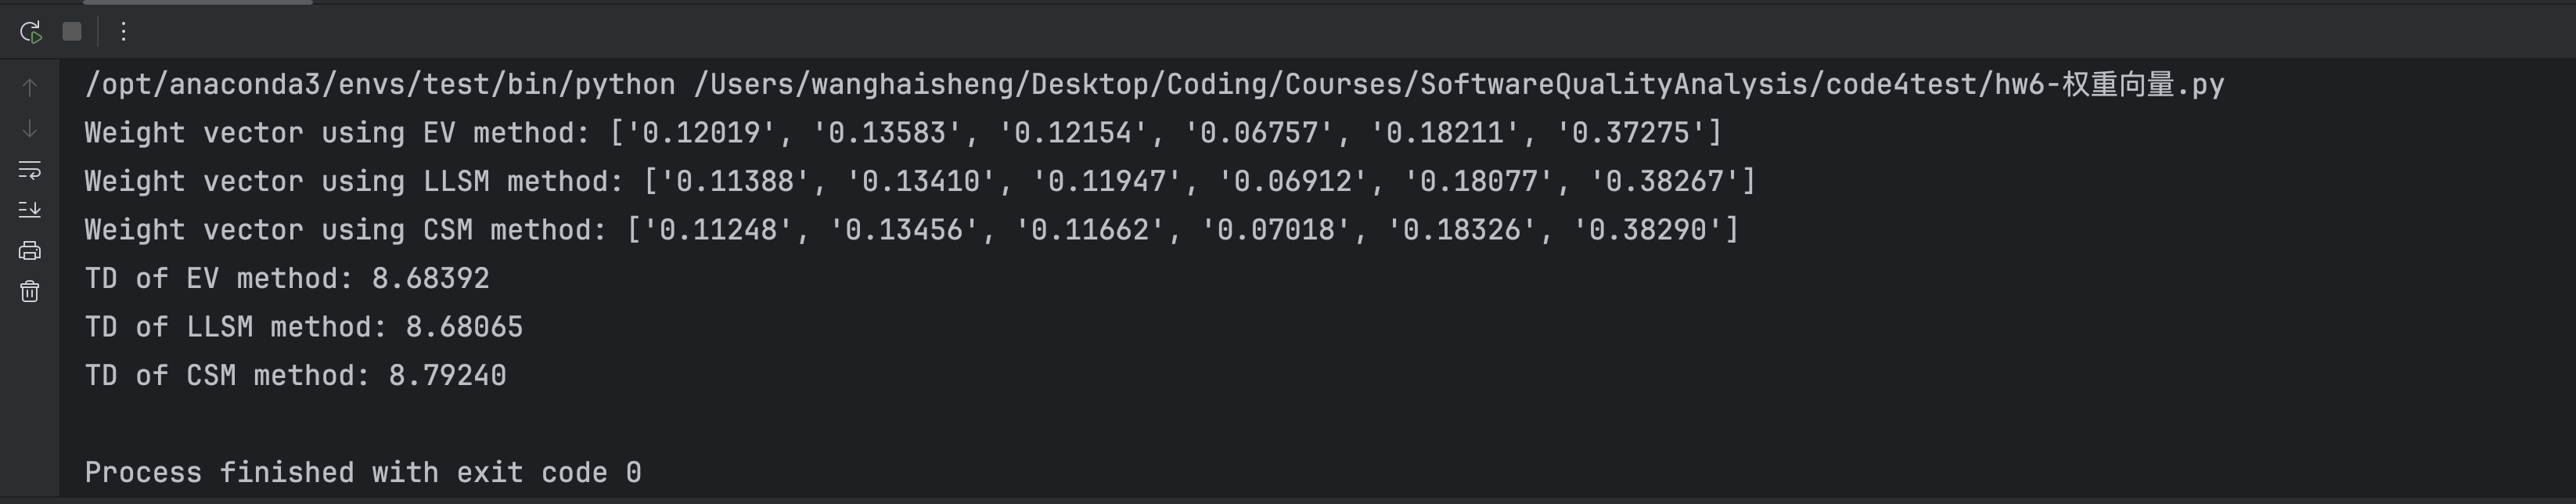
\includegraphics[width=0.9\textwidth]{img/01.png}
	\caption{运行结果}
\end{figure}

\subsubsection{题目答案}

\textbf{权重向量:}

Weight vector using EV method: ['0.12019', '0.13583', '0.12154', '0.06757', '0.18211', '0.37275']

Weight vector using LLSM method: ['0.11388', '0.13410', '0.11947', '0.06912', '0.18077', '0.38267']

Weight vector using CSM method: ['0.11248', '0.13456', '0.11662', '0.07018', '0.18326', '0.38290']

\textbf{“强度”TD计算:}

TD of EV method: 8.68392

TD of LLSM method: 8.68065

TD of CSM method: 8.79240

最终选择TD值最小的方法,即LLSM对应的8.68065。











\section{第二题}

\subsection{相关知识点}

\begin{figure}[H]
	\centering
	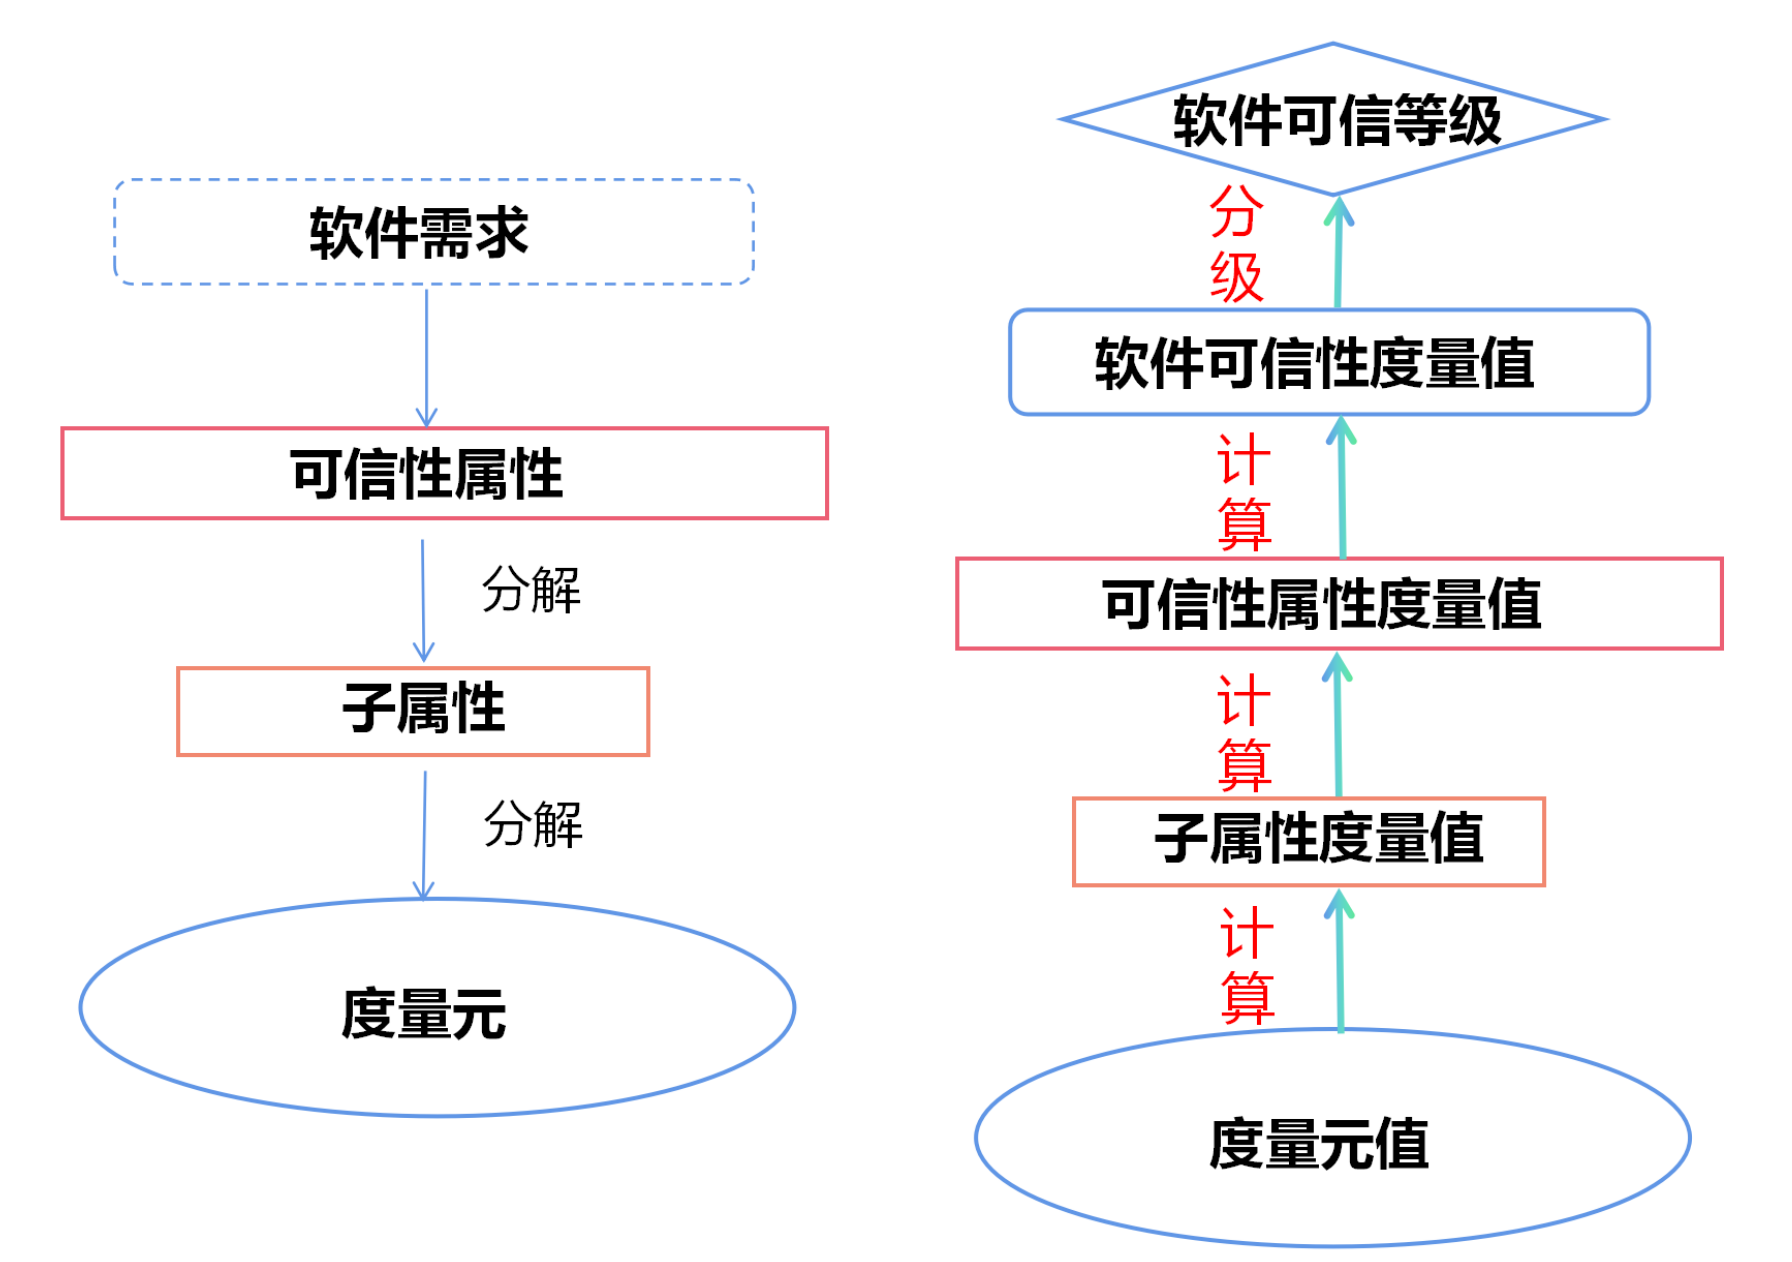
\includegraphics[width=0.6\textwidth]{img/static_1.png}
\end{figure}

由课堂内容可知,分析一个软件的可信等级,需要先自上而下地将软件需求解构为可信性属性、子属性、度量元;在计算时,要自下而上地计算每一个子类,然后得到最终的可信等级。更细节的流程图如下所示。

\begin{figure}[H]
	\centering
	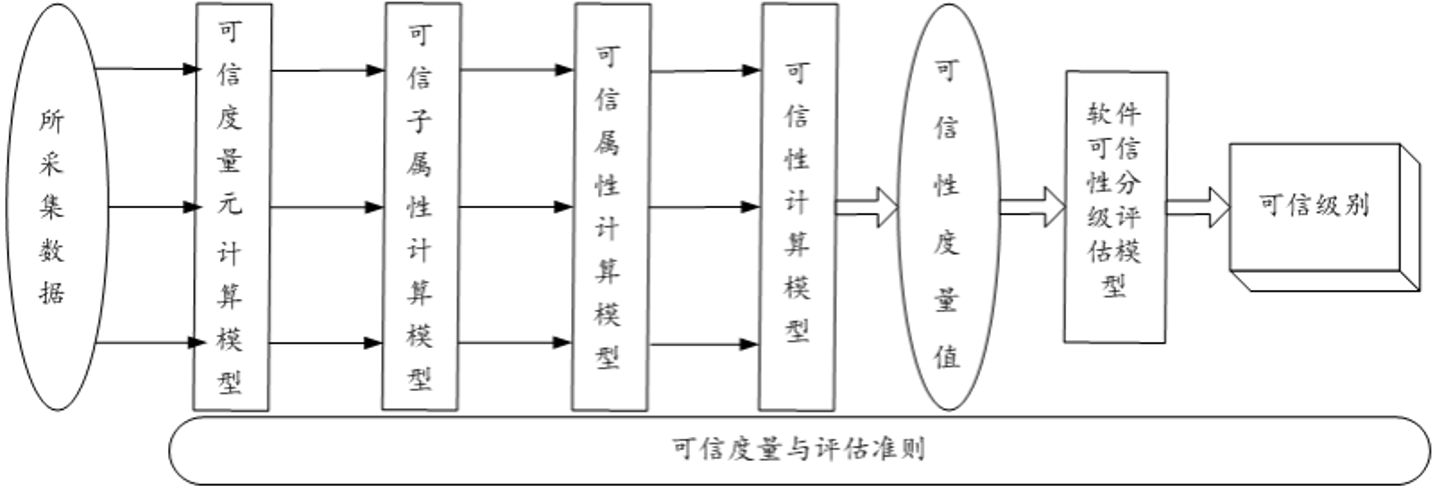
\includegraphics[width=0.9\textwidth]{img/static_2.png}
\end{figure}

在最后一步,通过下述分级模型来判定软件可信等级。

\begin{center}
	\begin{tabular}{|l|l|c|}
		\hline
		\textbf{软件可信度量值要求(黄金分割)} & \textbf{可信属性要求(多数原则)} & \textbf{可信等级} \\ \hline
		$9.5 \leq T$ & 
		\begin{tabular}[c]{@{}l@{}}1. 低于9.5分的关键属性个数不超过 $n - \left\lceil n \cdot \frac{2}{3} \right\rceil$ 个 \\ 2. 没有低于8.5分的可信属性\end{tabular} & V \\ \hline
		\begin{tabular}[c]{@{}l@{}}$8.5 \leq T < 9.5$ 或者 \\ $T > 9.5$ 且不能评为V级别\end{tabular} & 
		\begin{tabular}[c]{@{}l@{}}1. 低于8.5分的关键属性个数不超过 $n - \left\lceil n \cdot \frac{2}{3} \right\rceil$ 个 \\ 2. 没有低于7.0分的可信属性\end{tabular} & IV \\ \hline
		\begin{tabular}[c]{@{}l@{}}$7.0 \leq T < 8.5$ 或者 \\ $T > 8.5$ 且不能评为IV级别及以上者\end{tabular} & 
		\begin{tabular}[c]{@{}l@{}}1. 低于7.0分的关键属性个数不超过 $n - \left\lceil n \cdot \frac{2}{3} \right\rceil$ 个 \\ 2. 没有低于4.5分的可信属性\end{tabular} & III \\ \hline
		\begin{tabular}[c]{@{}l@{}}$4.5 \leq T < 7.0$ 或者 \\ $T > 7.0$ 且不能评为III级别及以上者\end{tabular} & 
		\begin{tabular}[c]{@{}l@{}}1. 低于4.5分的关键属性个数不超过 $n - \left\lceil n \cdot \frac{2}{3} \right\rceil$ 个\end{tabular} & II \\ \hline
		\begin{tabular}[c]{@{}l@{}}$T < 4.5$ 或者 \\ $T > 4.5$ 且不能评为II级别及以上者\end{tabular} & 
		1. 无要求 & I \\ \hline
	\end{tabular}
\end{center}

\subsection{答案}

\subsubsection{代码运行结果}

\begin{figure}[H]
	\centering
	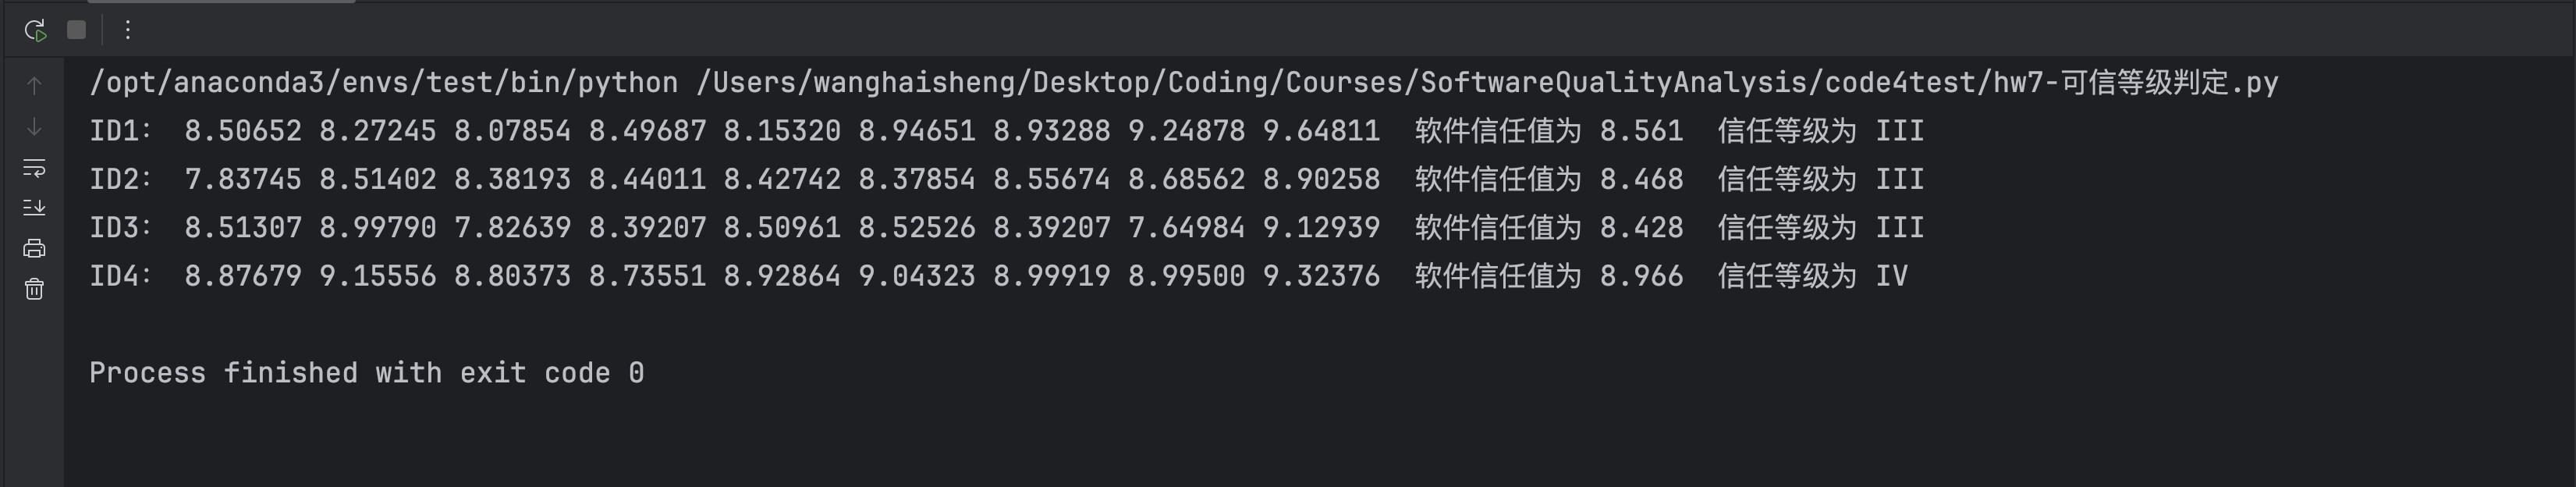
\includegraphics[width=0.9\textwidth]{img/02.png}
	\caption{运行结果}
\end{figure}

\subsubsection{题目答案}

ID1: 8.50652 8.27245 8.07854 8.49687 8.15320 8.94651 8.93288 9.24878 9.64811  软件信任值为 8.561  信任等级为 III

ID2: 7.83745 8.51402 8.38193 8.44011 8.42742 8.37854 8.55674 8.68562 8.90258  软件信任值为 8.468  信任等级为 III

ID3: 8.51307 8.99790 7.82639 8.39207 8.50961 8.52526 8.39207 7.64984 9.12939  软件信任值为 8.428  信任等级为 III

ID4: 8.87679 9.15556 8.80373 8.73551 8.92864 9.04323 8.99919 8.99500 9.32376  软件信任值为 8.966  信任等级为 IV

\subsubsection{可视化效果}

\begin{figure}[H]
	\centering
	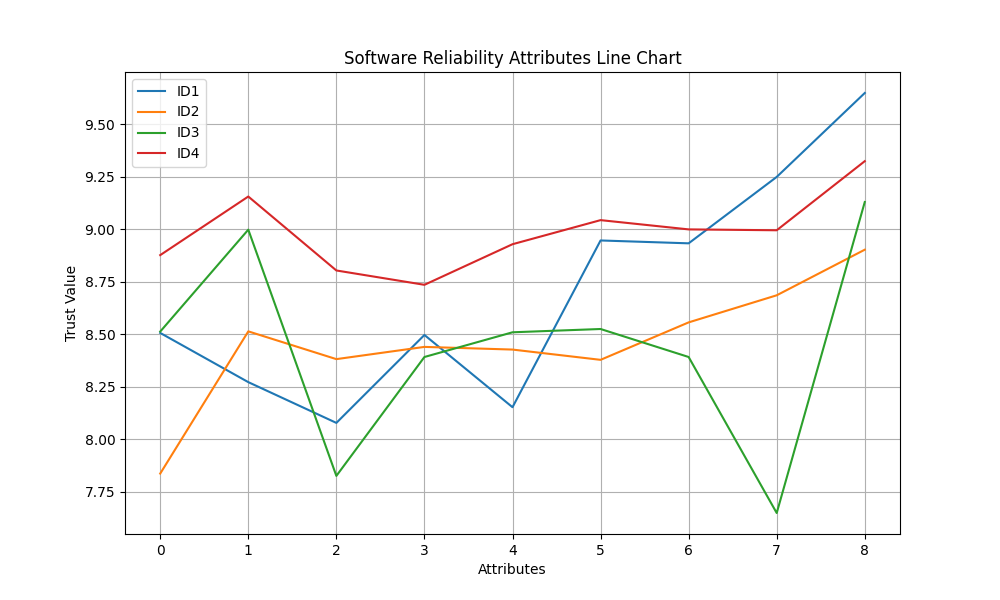
\includegraphics[width=0.9\textwidth]{img/0201.png}
	\caption{软件可信属性折线图}
\end{figure}

\begin{figure}[H]
	\centering
	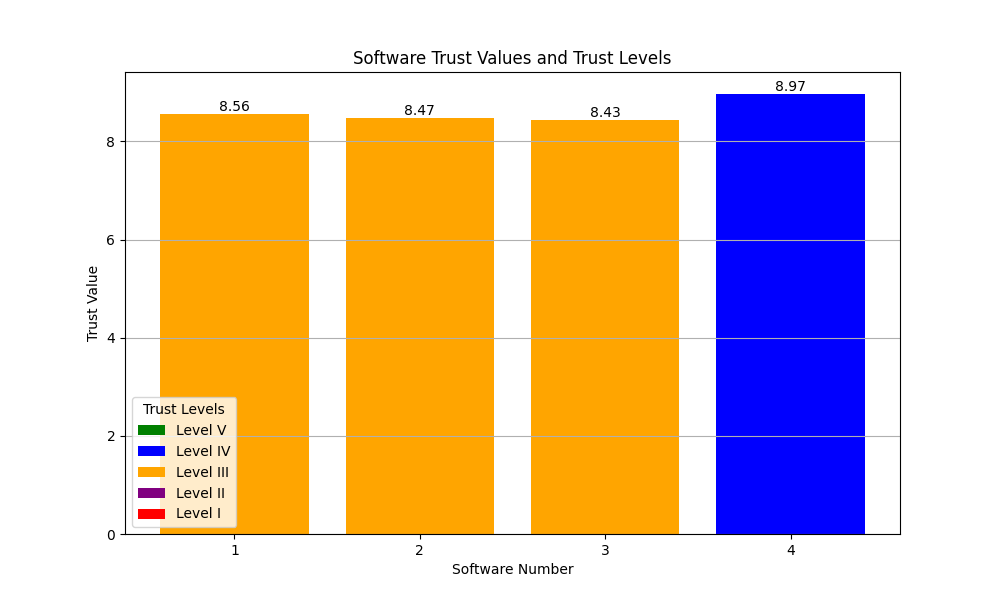
\includegraphics[width=0.9\textwidth]{img/0202.png}
	\caption{软件可信等级柱状图}
\end{figure}







\section{第三题}

\subsection{相关知识点}

\begin{figure}[H]
	\centering
	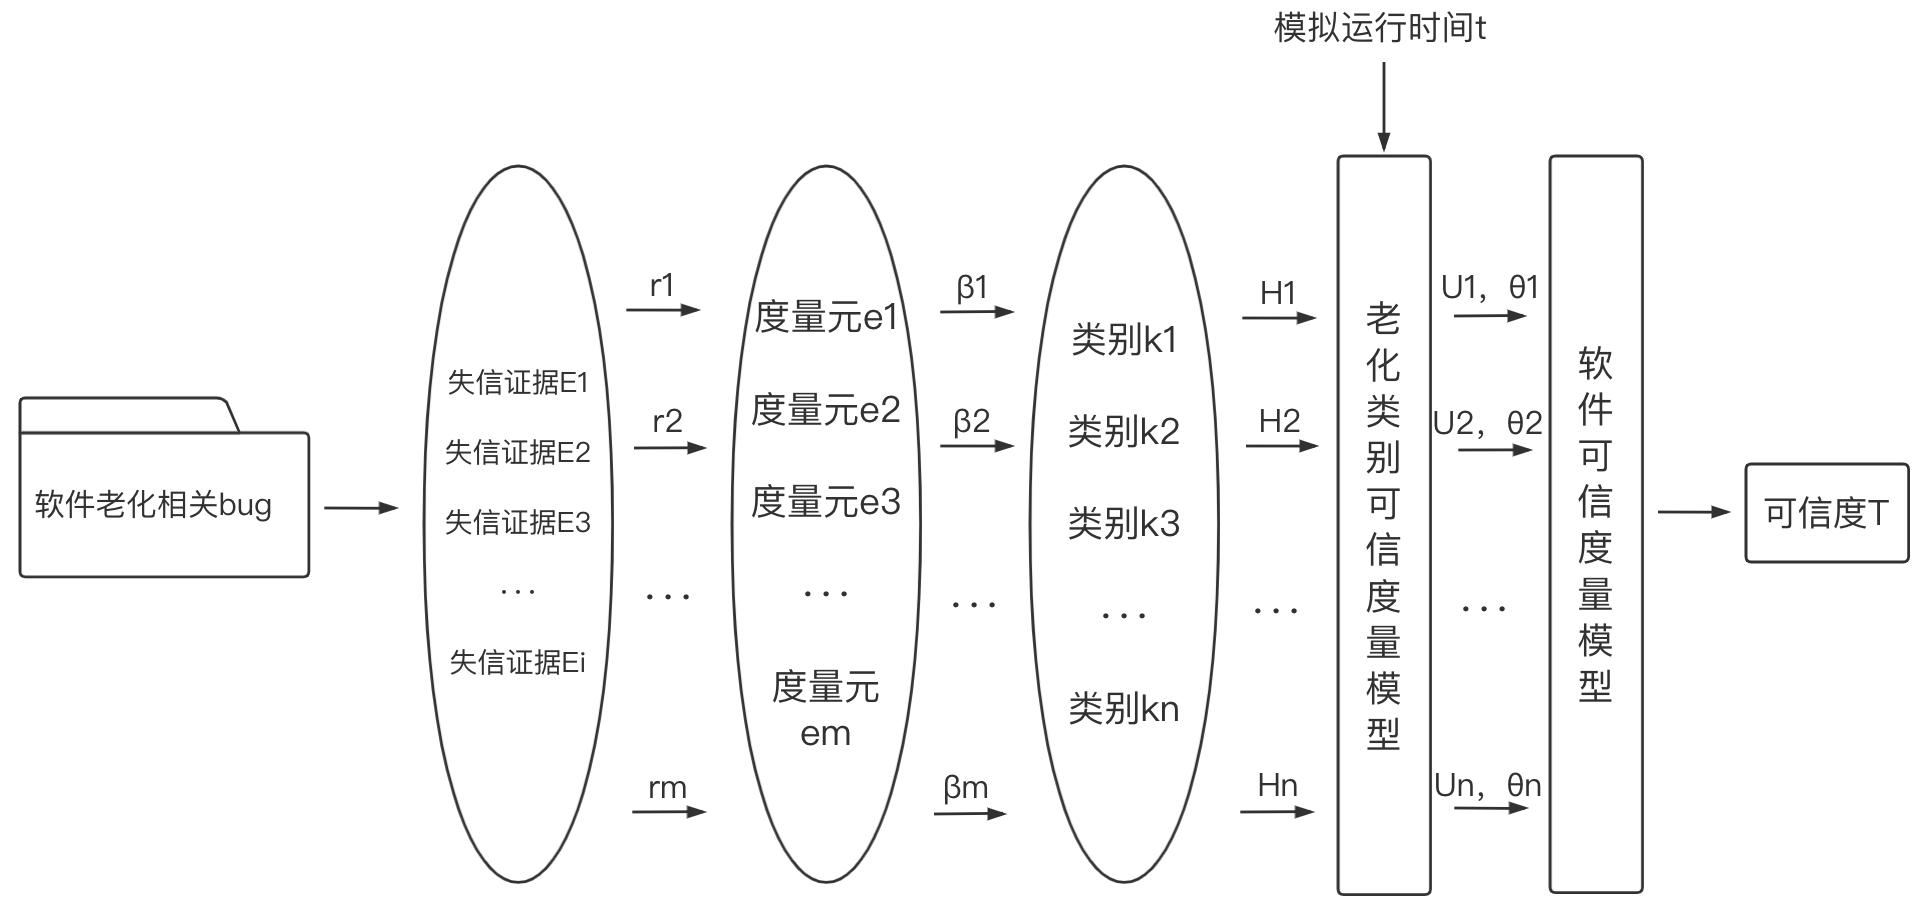
\includegraphics[width=0.9\textwidth]{img/static_3.png}
	\caption{软件老化可信计算框架}
\end{figure}

\subsection{答案}

\subsubsection{代码运行结果}

\begin{figure}[H]
	\centering
	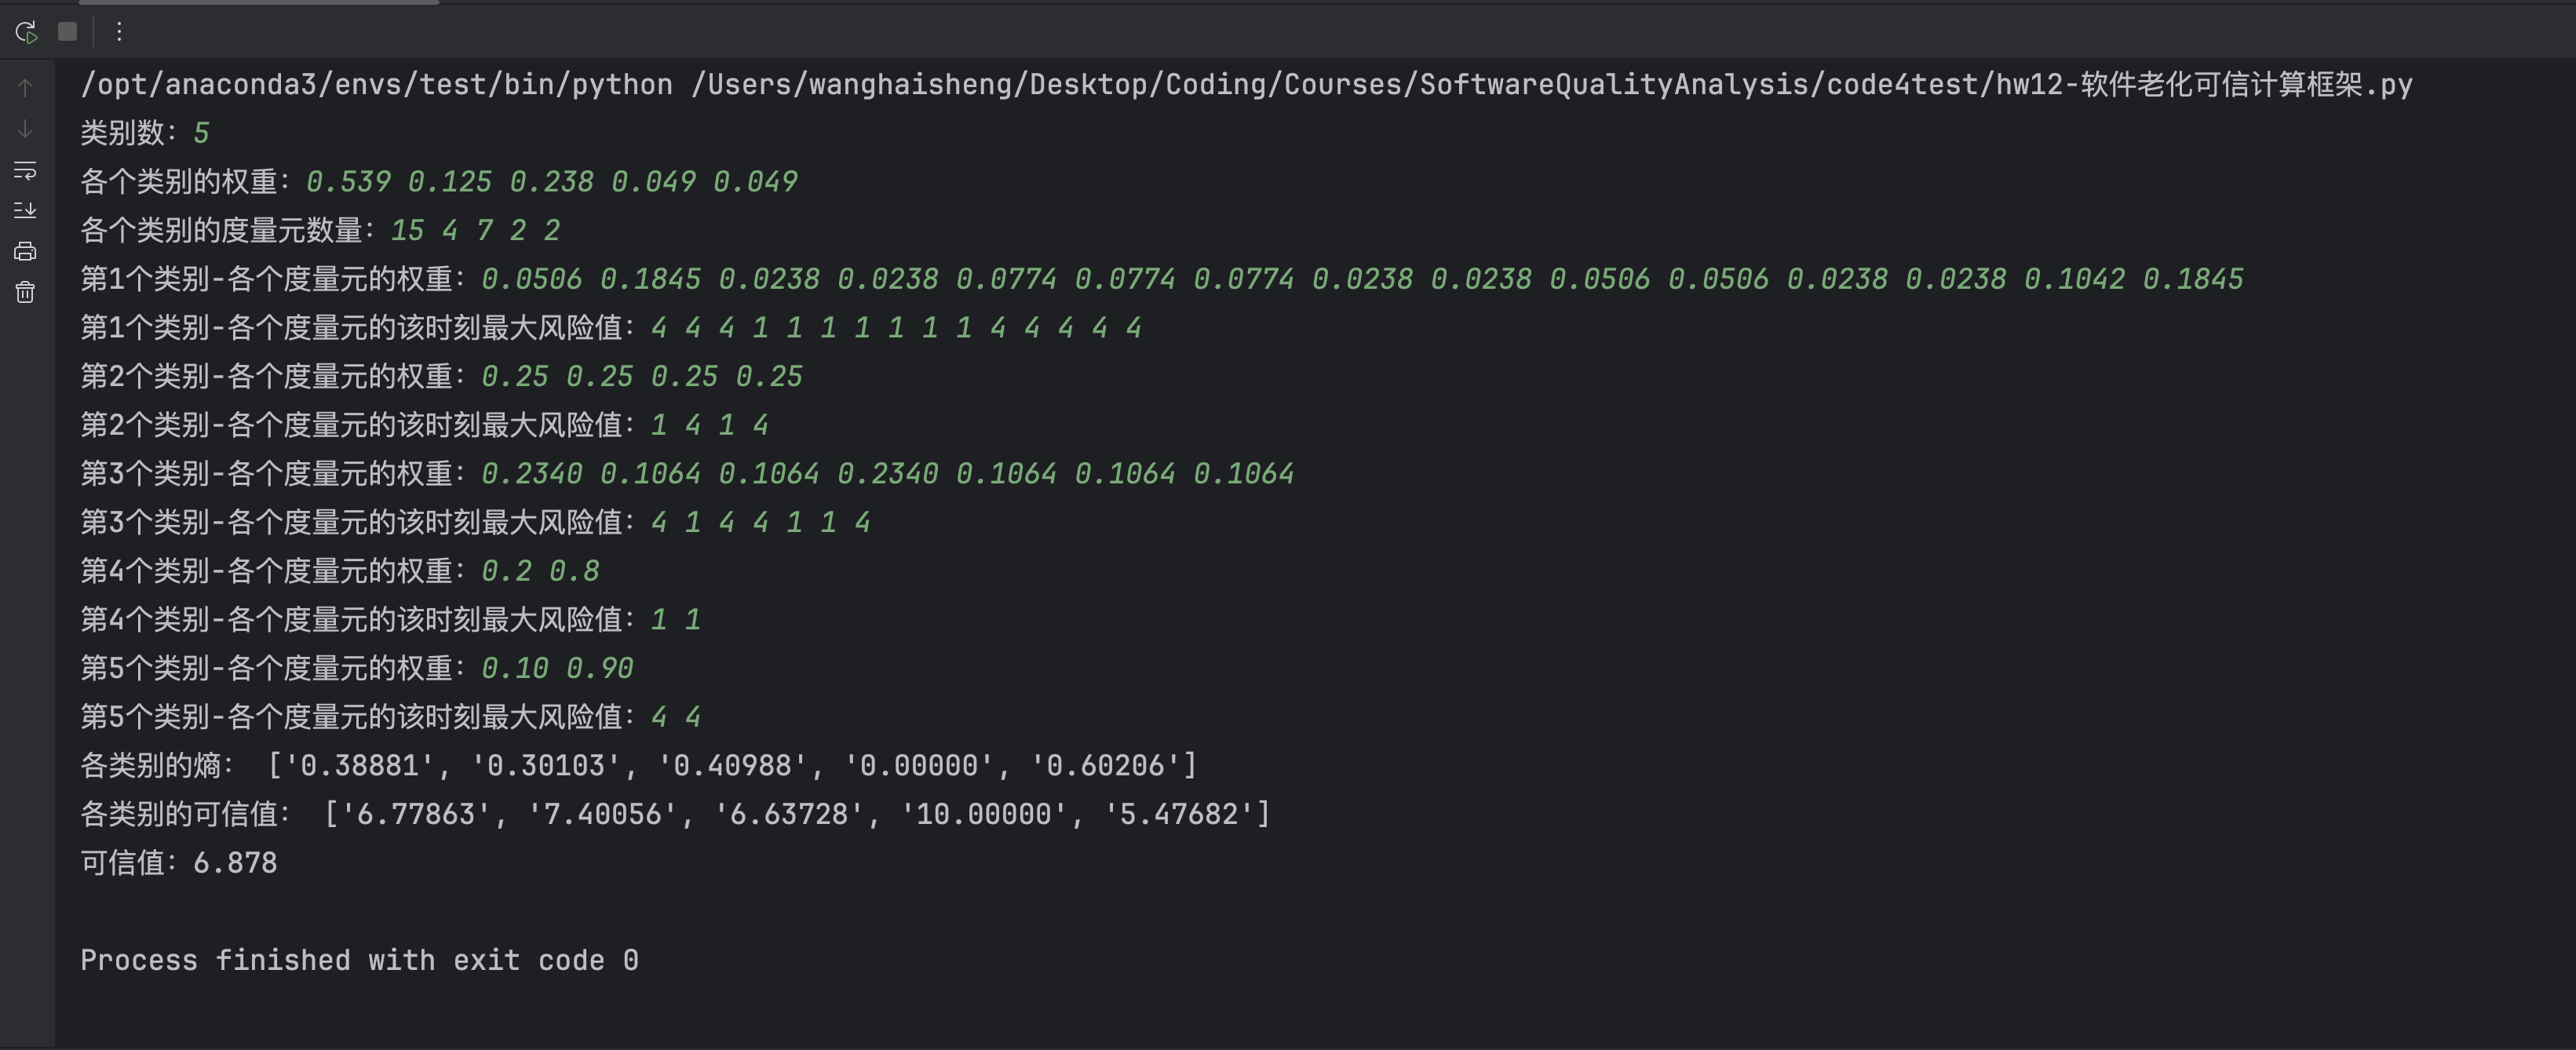
\includegraphics[width=0.9\textwidth]{img/0301.png}
	\caption{\texttt{t = 0}运行结果}
\end{figure}

\begin{figure}[H]
	\centering
	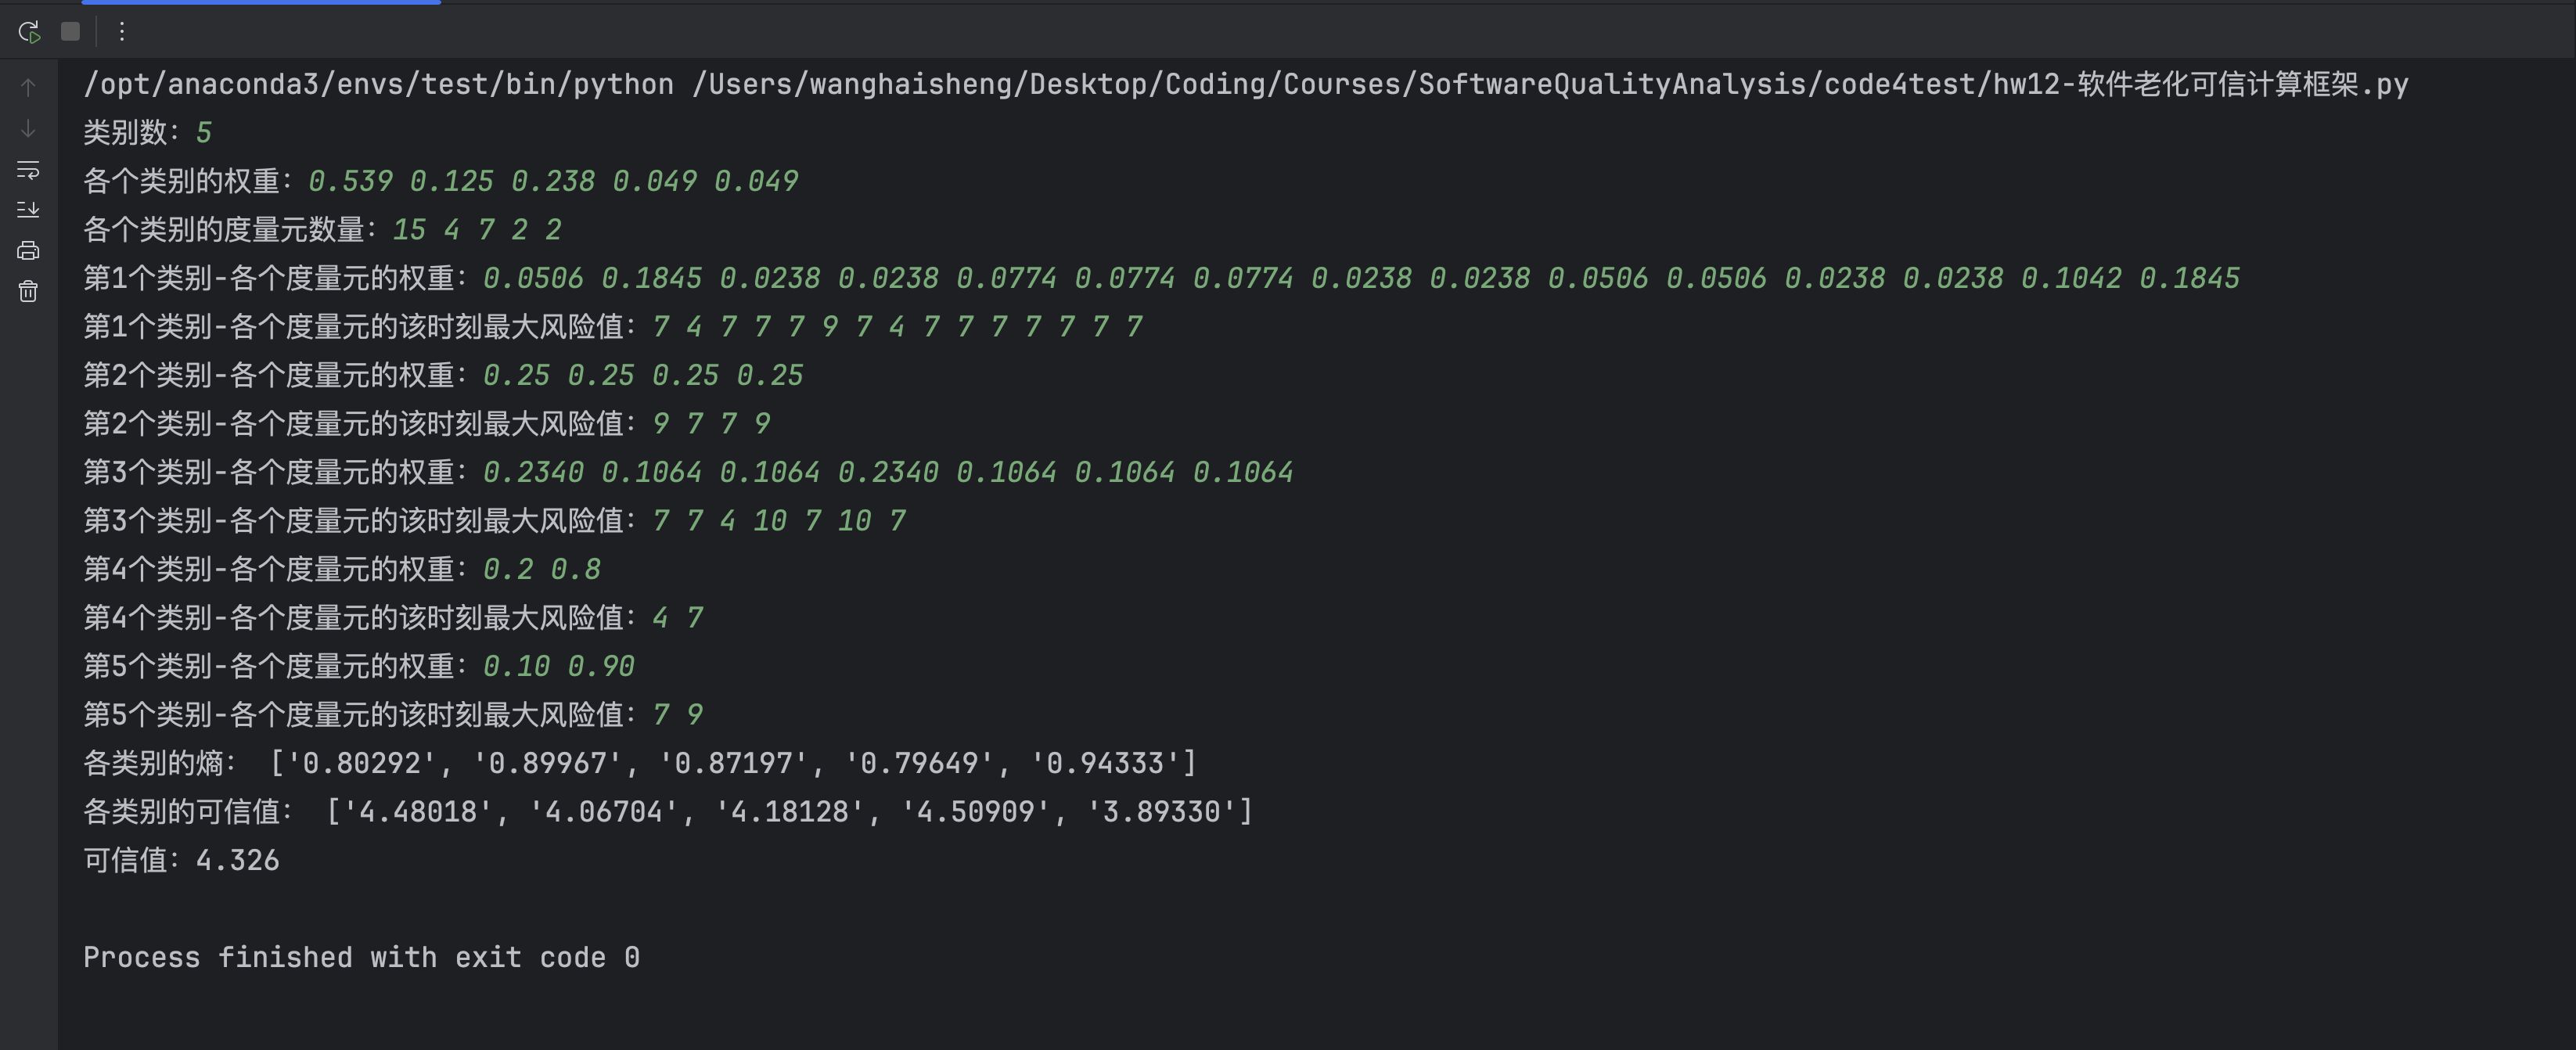
\includegraphics[width=0.9\textwidth]{img/0302.png}
	\caption{\texttt{t = 10}运行结果}
\end{figure}

\subsubsection{题目答案}

t = 0时:

各类别的熵: ['0.38881', '0.30103', '0.40988', '0.00000', '0.60206']
各类别的可信值: ['6.77863', '7.40056', '6.63728', '10.00000', '5.47682']
可信值:6.878

t = 10时:

各类别的熵: ['0.80292', '0.89967', '0.87197', '0.79649', '0.94333']
各类别的可信值: ['4.48018', '4.06704', '4.18128', '4.50909', '3.89330']
可信值:4.326

\section{附录:源代码}

\subsection{第一题}

\begin{lstlisting}[language=Python]
	import numpy as np
	
	
	# 定义正互反判断矩阵A
	A = np.array([
	[1, 1/2, 2, 2, 1/2, 1/4],
	[2, 1 ,1, 2, 1/2, 1/3],
	[1/2, 1, 1, 2, 1, 1/3],
	[1/2, 1/2, 1/2, 1, 1/2, 1/5],
	[2, 2, 1, 2, 1, 1/2],
	[4, 3, 3, 5, 2, 1]
	])
	
	n = len(A)
	
	# EV方法
	def ev_method(A):
	eigenvalues, eigenvectors = np.linalg.eig(A)
	max_eigenvalue_index = np.argmax(eigenvalues.real)
	principal_eigenvector = eigenvectors[:, max_eigenvalue_index].real
	normalized_weights = principal_eigenvector / np.sum(principal_eigenvector)
	return normalized_weights
	
	# LLSM方法
	def lls_method(A):
	n = len(A)
	product_list = []
	for i in range(n):
	product = 1
	for j in range(n):
	if A[i][j] == 0:
	raise ValueError("Matrix element is zero.")
	product *= A[i][j]
	product_list.append(product**(1/n))
	sum_product = sum(product_list)
	weights = [product / sum_product for product in product_list]
	return list(map(float, weights))
	
	
	def csm_method(A, epsilon=1e-10, max_iter=1000):
	n = len(A)
	w = np.ones(n) / n  # Initial weight vector
	
	for iteration in range(max_iter):
	max_val, m = None, None
	
	# Step 1: Find the index `m` with the largest discrepancy
	for i in range(n):
	discrepancy = 0
	for j in range(n):
	discrepancy += ((1 + A[j, i] ** 2) * (w[i] / w[j]) - (1 + A[i, j] ** 2) * (w[j] / w[i]))
	discrepancy = abs(discrepancy)
	if max_val is None or discrepancy > max_val:
	max_val = discrepancy
	m = i
	
	# Step 2: Check for convergence
	if max_val <= epsilon:
	break
	
	# Step 3: Update the weight w[m]
	up, bottom = 0, 0
	for j in range(n):
	if j != m:
	up += (1 + A[m, j] ** 2) * (w[j] / w[m])
	bottom += (1 + A[j, m] ** 2) * (w[m] / w[j])
	
	# Update weight vector
	T = np.sqrt(up / bottom)
	w[m] *= T
	w /= np.sum(w)  # Normalize weights
	
	return w
	
	
	# 计算每种方法的权重向量
	W_EV = ev_method(A)
	W_LLSM = lls_method(A)
	W_CSM = csm_method(A)
	
	# 打印权重向量
	print("Weight vector using EV method:", [f"{w:.5f}" for w in W_EV])
	print("Weight vector using LLSM method:", [f"{w:.5f}" for w in W_LLSM])
	print("Weight vector using CSM method:", [f"{w:.5f}" for w in W_CSM])
	
	# 计算TD(Total Deviation)
	def total_deviation(W, A):
	n = len(A)
	TD = 0
	for i in range(n):
	for j in range(n):
	TD += abs(A[i][j] - W[i] / W[j])
	return TD
	
	
	TD_EV = total_deviation(W_EV, A)
	TD_LLSM = total_deviation(W_LLSM, A)
	TD_CSM = total_deviation(W_CSM, A)
	
	# 打印总偏差(TD)
	print("TD of EV method: {:.5f}".format(TD_EV))
	print("TD of LLSM method: {:.5f}".format(TD_LLSM))
	print("TD of CSM method: {:.5f}".format(TD_CSM))
	
	# 最终应当选择TD值最小的方法
	
\end{lstlisting}

\subsection{第二题}

\begin{lstlisting}[language=Python]
	import math
	import matplotlib.pyplot as plt
	
	
	# 权重
	weight = [0.05, 0.17, 0.20, 0.15, 0.09, 0.09, 0.11, 0.05, 0.09]
	
	# 子权重
	childWeight = [
	0.31, 0.36, 0.33,  # 指标1子权重
	0.33, 0.33, 0.34,  # 指标2子权重
	0.16, 0.17, 0.17, 0.17, 0.17, 0.16,  # 指标3子权重
	0.33, 0.34, 0.33,  # 指标4子权重
	0.34, 0.33, 0.33,  # 指标5子权重
	0.5, 0.5,          # 指标6子权重
	0.33, 0.34, 0.33,  # 指标7子权重
	0.5, 0.5,         # 指标8子权重
	0.33, 0.33, 0.34   # 指标9子权重
	]
	
	
	
	# 计算可信值
	def calculate_trust(values, weights):
	trust_value = 1.0
	for i in range(len(values)):
	trust_value *= math.pow(values[i], weights[i])
	return trust_value
	
	# 判断可信等级
	def judge_trust_level_07(component_trust_values, key_component_count, overall_trust):
	total_components = len(component_trust_values)
	key_threshold = 3
	low_key_count9_5 = 0
	low_key_count8_5 = 0
	low_key_count7_0 = 0
	low_key_count4_5 = 0
	has_low85 = False
	has_low70 = False
	has_low45 = False
	
	# 统计关键组件低于对应阈值的数量
	for i in range(key_component_count):
	if component_trust_values[i] < 9.5:
	low_key_count9_5 += 1
	if component_trust_values[i] < 8.5:
	low_key_count8_5 += 1
	if component_trust_values[i] < 7.0:
	low_key_count7_0 += 1
	if component_trust_values[i] < 4.5:
	low_key_count4_5 += 1
	
	# 统计所有组件低于对应阈值的情况
	for i in range(total_components):
	if component_trust_values[i] < 8.5:
	has_low85 = True
	if component_trust_values[i] < 7.0:
	has_low70 = True
	if component_trust_values[i] < 4.5:
	has_low45 = True
	
	# 判断信任等级
	if overall_trust >= 9.5 and low_key_count9_5 <= key_threshold and not has_low85:
	return "V"
	elif overall_trust >= 8.5 and not has_low70 and low_key_count8_5 <= key_threshold:
	return "IV"
	elif overall_trust >= 7.0 and not has_low45 and low_key_count7_0 <= key_threshold:
	return "III"
	elif overall_trust >= 4.5 and low_key_count4_5 <= key_threshold:
	return "II"
	else:
	return "I"
	
	# 绘制折线图
	def plot_line_chart(title, x_label, y_label, data, labels):
	plt.figure(figsize=(10, 6))
	for i, series in enumerate(data):
	plt.plot(series, label=labels[i])
	plt.title(title)
	plt.xlabel(x_label)
	plt.ylabel(y_label)
	plt.legend()
	plt.grid(True)
	plt.show()
	
	# 绘制条形图
	def plot_bar_chart(software_numbers, trust_values, trust_levels):
	# 定义等级对应的颜色
	level_colors = {
		"V": "green",
		"IV": "blue",
		"III": "orange",
		"II": "purple",
		"I": "red"
	}
	
	# 获取每个软件对应的颜色
	colors = [level_colors[level] for level in trust_levels]
	
	plt.figure(figsize=(10, 6))
	bars = plt.bar(software_numbers, trust_values, color=colors)
	
	# 添加数值标签
	for bar in bars:
	height = bar.get_height()
	plt.text(bar.get_x() + bar.get_width() / 2, height, f"{height:.2f}", ha='center', va='bottom')
	
	plt.title("Software Trust Values and Trust Levels")
	plt.xlabel("Software Number")
	plt.ylabel("Trust Value")
	plt.xticks(software_numbers)
	plt.grid(True, axis='y')
	
	# 添加图例
	from matplotlib.patches import Patch
	legend_elements = [
	Patch(facecolor='green', label='Level V'),
	Patch(facecolor='blue', label='Level IV'),
	Patch(facecolor='orange', label='Level III'),
	Patch(facecolor='purple', label='Level II'),
	Patch(facecolor='red', label='Level I')
	]
	plt.legend(handles=legend_elements, title="Trust Levels")
	
	plt.show()
	
	# 主函数
	def main():
	# 4组28个子属性平均值
	child_trust_values_list = [
	[9.1, 8.9, 7.6, 9.2, 7.8, 7.9, 8.9, 7.8, 7.9, 7.6, 7.5, 9.0, 9.1, 7.6, 8.9, 9.0, 7.9, 7.6, 9.2, 8.7, 8.9, 8.9, 9.0, 9.1, 9.4, 10, 10, 9.0],
	[7.7, 7.9, 7.9, 9.0, 8.7, 7.9, 8.7, 8.2, 8.7, 8.2, 7.7, 8.9, 9.0, 7.7, 8.7, 8.7, 7.9, 8.7, 9.0, 7.8, 7.9, 8.9, 8.9, 9.2, 8.2, 8.9, 7.9, 10],
	[7.9, 8.9, 8.7, 9.2, 8.9, 8.9, 7.9, 7.9, 8.7, 6.2, 7.9, 8.7, 8.7, 8.7, 7.8, 7.8, 8.9, 8.9, 9.2, 7.9, 8.7, 8.7, 7.8, 7.7, 7.6, 9.3, 9.2, 8.9],
	[8.7, 9.2, 8.7, 9.3, 9.5, 8.7, 8.7, 9.3, 8.7, 7.7, 8.9, 9.7, 9.7, 8.7, 7.9, 8.7, 8.9, 9.2, 9.4, 8.7, 8.9, 9.4, 8.7, 8.7, 9.3, 9.5, 9.6, 8.9]
	]
	
	# 处理每一组数据
	attribute_trust_values_list = []
	software_trust_values = []
	trust_levels = []
	
	for i in range(len(child_trust_values_list)):
	child_trust_values = child_trust_values_list[i]
	
	# 计算各属性信任值
	attribute_trust_values = []
	index = 0
	for attr in range(len(weight)):
	sub_trusts = []
	sub_weights = []
	if attr == 0:
	sub_trusts = [child_trust_values[index], child_trust_values[index+1], child_trust_values[index+2]]
	index += 3
	elif attr == 1:
	sub_trusts = [child_trust_values[index], child_trust_values[index+1], child_trust_values[index+2]]
	index += 3
	elif attr == 2:
	sub_trusts = [child_trust_values[index], child_trust_values[index+1], child_trust_values[index+2],
	child_trust_values[index+3], child_trust_values[index+4], child_trust_values[index+5]]
	index += 6
	elif attr == 3:
	sub_trusts = [child_trust_values[index], child_trust_values[index+1], child_trust_values[index+2]]
	index += 3
	elif attr == 4:
	sub_trusts = [child_trust_values[index], child_trust_values[index+1], child_trust_values[index+2]]
	index += 3
	elif attr == 5:
	sub_trusts = [child_trust_values[index], child_trust_values[index+1]]
	index += 2
	elif attr == 6:
	sub_trusts = [child_trust_values[index], child_trust_values[index+1], child_trust_values[index+2]]
	index += 3
	elif attr == 7:
	sub_trusts = [child_trust_values[index], child_trust_values[index+1]]
	index += 2
	elif attr == 8:
	sub_trusts = [child_trust_values[index], child_trust_values[index+1], child_trust_values[index+2]]
	index += 3
	
	sub_weights = childWeight[index-len(sub_trusts):index]
	attribute_trust_values.append(calculate_trust(sub_trusts, sub_weights))
	
	attribute_trust_values_list.append(attribute_trust_values)
	
	# 计算软件信任值
	software_trust_value = calculate_trust(attribute_trust_values, weight)
	software_trust_values.append(software_trust_value)
	
	# 判断信任等级
	trust_level = judge_trust_level_07(attribute_trust_values, len(attribute_trust_values), software_trust_value)
	trust_levels.append(trust_level)
	
	# 输出每组的各属性信任值
	print(f"ID{i + 1}:", end=" ")
	for attr_trust in attribute_trust_values:
	print(f"{attr_trust:.5f}", end=" ")
	
	# 输出软件信任值及信任等级
	print(f" 软件信任值为 {software_trust_value:.3f}  信任等级为 {trust_level}")
	
	# 可视化属性信任值
	labels = [f"ID{i + 1}" for i in range(len(child_trust_values_list))]
	plot_line_chart("Software Reliability Attributes Line Chart", "Attributes", "Trust Value", attribute_trust_values_list, labels)
	
	# 可视化软件信任值(条形图)
	software_numbers = range(1, 1 + len(child_trust_values_list))
	plot_bar_chart(software_numbers, software_trust_values, trust_levels)
	
	if __name__ == "__main__":
	main()
	
\end{lstlisting}

\subsection{第三题}

\begin{lstlisting}[language=Python]
	n = int(input("类别数:"))
	theta = list(map(float, input("各个类别的权重:").split()))
	m = list(map(int, input("各个类别的度量元数量:").split()))
	R = []
	BETA = []
	for i in range(n):
	beta = list(map(float, input("第{0}个类别-各个度量元的权重:".format(i + 1)).split()))
	r = list(map(float, input("第{0}个类别-各个度量元的该时刻最大风险值:".format(i + 1)).split()))
	BETA.append(beta)
	R.append(r)
	
	import math
	Hs = []
	Us = []
	for i in range(n):
	H = 0
	for j in range(m[i]):
	H += BETA[i][j] * math.log10(R[i][j])
	U = max(10 * math.exp(-H), 1)
	Hs.append(H)
	Us.append(U)
	
	formatted_Hs = [f"{x:.5f}" for x in Hs]
	print("各类别的熵:", formatted_Hs)
	
	formatted_Us = [f"{x:.5f}" for x in Us]
	print("各类别的可信值:", formatted_Us)
	
	T = 1
	for i in range(n):
	T *= math.pow(Us[i], theta[i])
	print("可信值:{0:.3f}".format(T))
	
	
\end{lstlisting}

\end{document}